
\toolName\  was developed as a  MATLAB~\cite{matlab} standalone application.
It is developed on top of an existing planner---presented in~\cite{tumova2016multi}---which has been chosen since it already implements a decentralized planning procedure.
\toolName\ calls this planner twice considering two different versions of the model of the robots and their environments. 
The results obtained by performing this procedure are sound and correct.
Additional details and proofs can be found in~\cite{menghi2018multi}.


\toolName\ can be executed in two ways, as shown in Listing~\ref{lst:command}.
The first option is used to compute plans for custom missions in custom models of environment and robots.
\texttt{robots} is a variable that specifies the number of robots and their models.
Then, \texttt{environment} is a variable that contains a model of the environment and its uncertainty.
Finally, \texttt{missions} contains the local mission to be achieved by each robot.
With the second option, we provide a way of replicating the experiments presented in this paper and in~\cite{menghi2018multi}.
\texttt{Scenario} is a Matlab file containing the model of the environment and the robots and \texttt{Experiment} encodes the mission that must be satisfied by each robot.
Then, \texttt{Location} defines where the experiments are allocated---i.e., RQ1, RQ2, or RunningExample.



\begin{lstlisting}[frame=single, backgroundcolor=\color{light-gray}, basicstyle=\footnotesize\ttfamily, language=Java, numbers=left, numberstyle=\tiny\color{black},caption= {Running \toolName}\label{lst:command}, captionpos=b]
mapmakerRunner(robots, environment , missions);
mapmaker_exp('Scenario', 'Experiment', 'Location')
\end{lstlisting}

%The tool is composed by several MATLAB-based scripts that can be executed independently for performing certain functions.
%In order to use \toolName it is sufficient to launch the function \emph{mapmaker\_exp} where the \emph{research question}, the \emph{example} or map of the environment and the \emph{experiment} to check are their arguments.
%This function enormously simplifies the performance of the tool, but there are other functionalities that can also be exploited explained in the previous section.





%In a normal case where the scenarios are already defined, the only components of the architecture depicted in~\ref{fig:overview} that are used are the \emph{Replication Package}, the \emph{Robot \& Environment models with uncertainty}, the \emph{Planner} itself and its inputs and, of course, the \emph{Solutions container}.
%The first component represents a folder where the models of the robot and environment with a certain added uncertainty for the selected experiment are stored.

When  \toolName\ is executed a graphical interface similar to the one presented  in Figure~\ref{fig:outputexample} is showed.
The figure is a screenshot showing the performance of our tool where we changed the size of some numbers and added the plans for helping the reader.
The grid represents the environment in which the robots are moving.
Each cell represents a location of the environment and has a number associated, as labeled in some of them.
Robots are represented by squared colored boxes.
Actions are used to encode movements, i.e., each robot can move left, right, up, and down.
A robot  cannot move between adjacent cells if they are separated by thick bordered lines.
Whenever  it is unclear if a robot can move between adjacent cells, these cells are separated by a red border.
%Each service is associated with a number.
Whenever a service can be provided by a robot in a cell, the cell is labeled with the associated number and the color of the corresponding robot.
Finally, synchronization capabilities are represented by a black cross.
If it is unclear if two robots can synchronize in a cell, the cell is labeled with a green cross.
The graphical interface shows the plan execution.
Assume for example that the robots $r_1$, $r_2$, and $r_3$ have the following \emph{local missions}.
Robot $r_1$ has to perform service 1, which is provided in cells 7 and 9.
Service 1 and service 2 (which has to be accomplished by robot $r_2$) are located in a cell labeled with a cross, so robots must meet there and perform both actions at the same time.
Robot $r_1$ can also perform this mission in cell 9, but the synchronization in this cell is unsure.
Robot $r_2$ must synchronize with robot $r_1$ and perform service 2, but then it has to reach cell 22 for performing action 3.
Finally, robot $r_3$ has to perform service 4 in cell 2 and service 5 in cell 18 or in cell 30.

In Figure~\ref{fig:outputexample} we show different plans that can be performed by the robots. 
They all accomplish a number of actions in a periodic fashion.
Robot $r_1$ could accomplish two different plans.
P1 represents a definitive plan and P1' a possible plan where a true evidence was detected by the robot.
In both paths, the robot reaches the cell where the requested service can be performed with the help of robot $r_2$.
For robot $r_2$ we show two different paths as well.
P2 represents a possible plan ---due to the uncertainty of the transition between cells 14 and 20--- where $r_2$ must synchronize with $r_1$ in order to accomplish service 2.
P2' is a similar path with the difference that the synchronization is not assured in the associated cell.
Finally, P3 represents a possible path where robot $r_3$ accomplishes service 4 and service 5 in cell 18.

\sergio{use something like this in the previous paragraph}
The following missions were considered:
\begin{enumerate*}
	\item robot $r_1$ must achieve the mission $\Event (s_1 \wedge (\Event (s_2 \vee s_3) ))$. It had to reach a predefined destination where service  $s_1$ is provided, and then  perform either service $s_2$  or service $s_3$.
	%This is a variation of  the sequencing pattern~\cite{kress2009temporal,yoo2016online}, which requires to first visit a location where the service $s_1$ is provided and then visit a location where the service $s_2$ or $s_3$ is provided.
	\item robot $r_2$  must achieve the following mission $\Always(\Event(s_4 \vee s_5))$.
	Furthermore, it aims at helping $r_1$ in providing service  $s_1$, i.e., robots $r_1$ and $r_2$ must meet in cells where  service $s_1$ is provided.
	%This is a variation of the surveillance pattern~\cite{kress2009temporal,yoo2016online}, which requires to keep visiting locations where service $s_4$ or $s_5$ is provided.
\end{enumerate*}

%The results achieved and presented in~\cite{mapmaker17} can be replicated using this models.
%They are loaded and set as MATLAB workspace variables in the second component.

%The planner needs as input the information from this variables and also from the scripts \emph{Algorithms}, \emph{Utils} and \emph{Configuration files}, that are automatically linked.
%During the execution of the planner \sergio{image representing the execution of the tool?} the MATLAB interface shows a window with the goals of the current mission. 
%Furthermore, after the computation of the plan it shows the movements of the robots and their knowledge of the environment.
%When all the robots have reached their goals or they realized that their local mission is not feasible the experiments concludes.
%Once the experiment is concluded, the data extracted (as explained in~\ref{sec:approach}) is stored in the solutions container component.


\begin{figure}[t]
\begin{center}
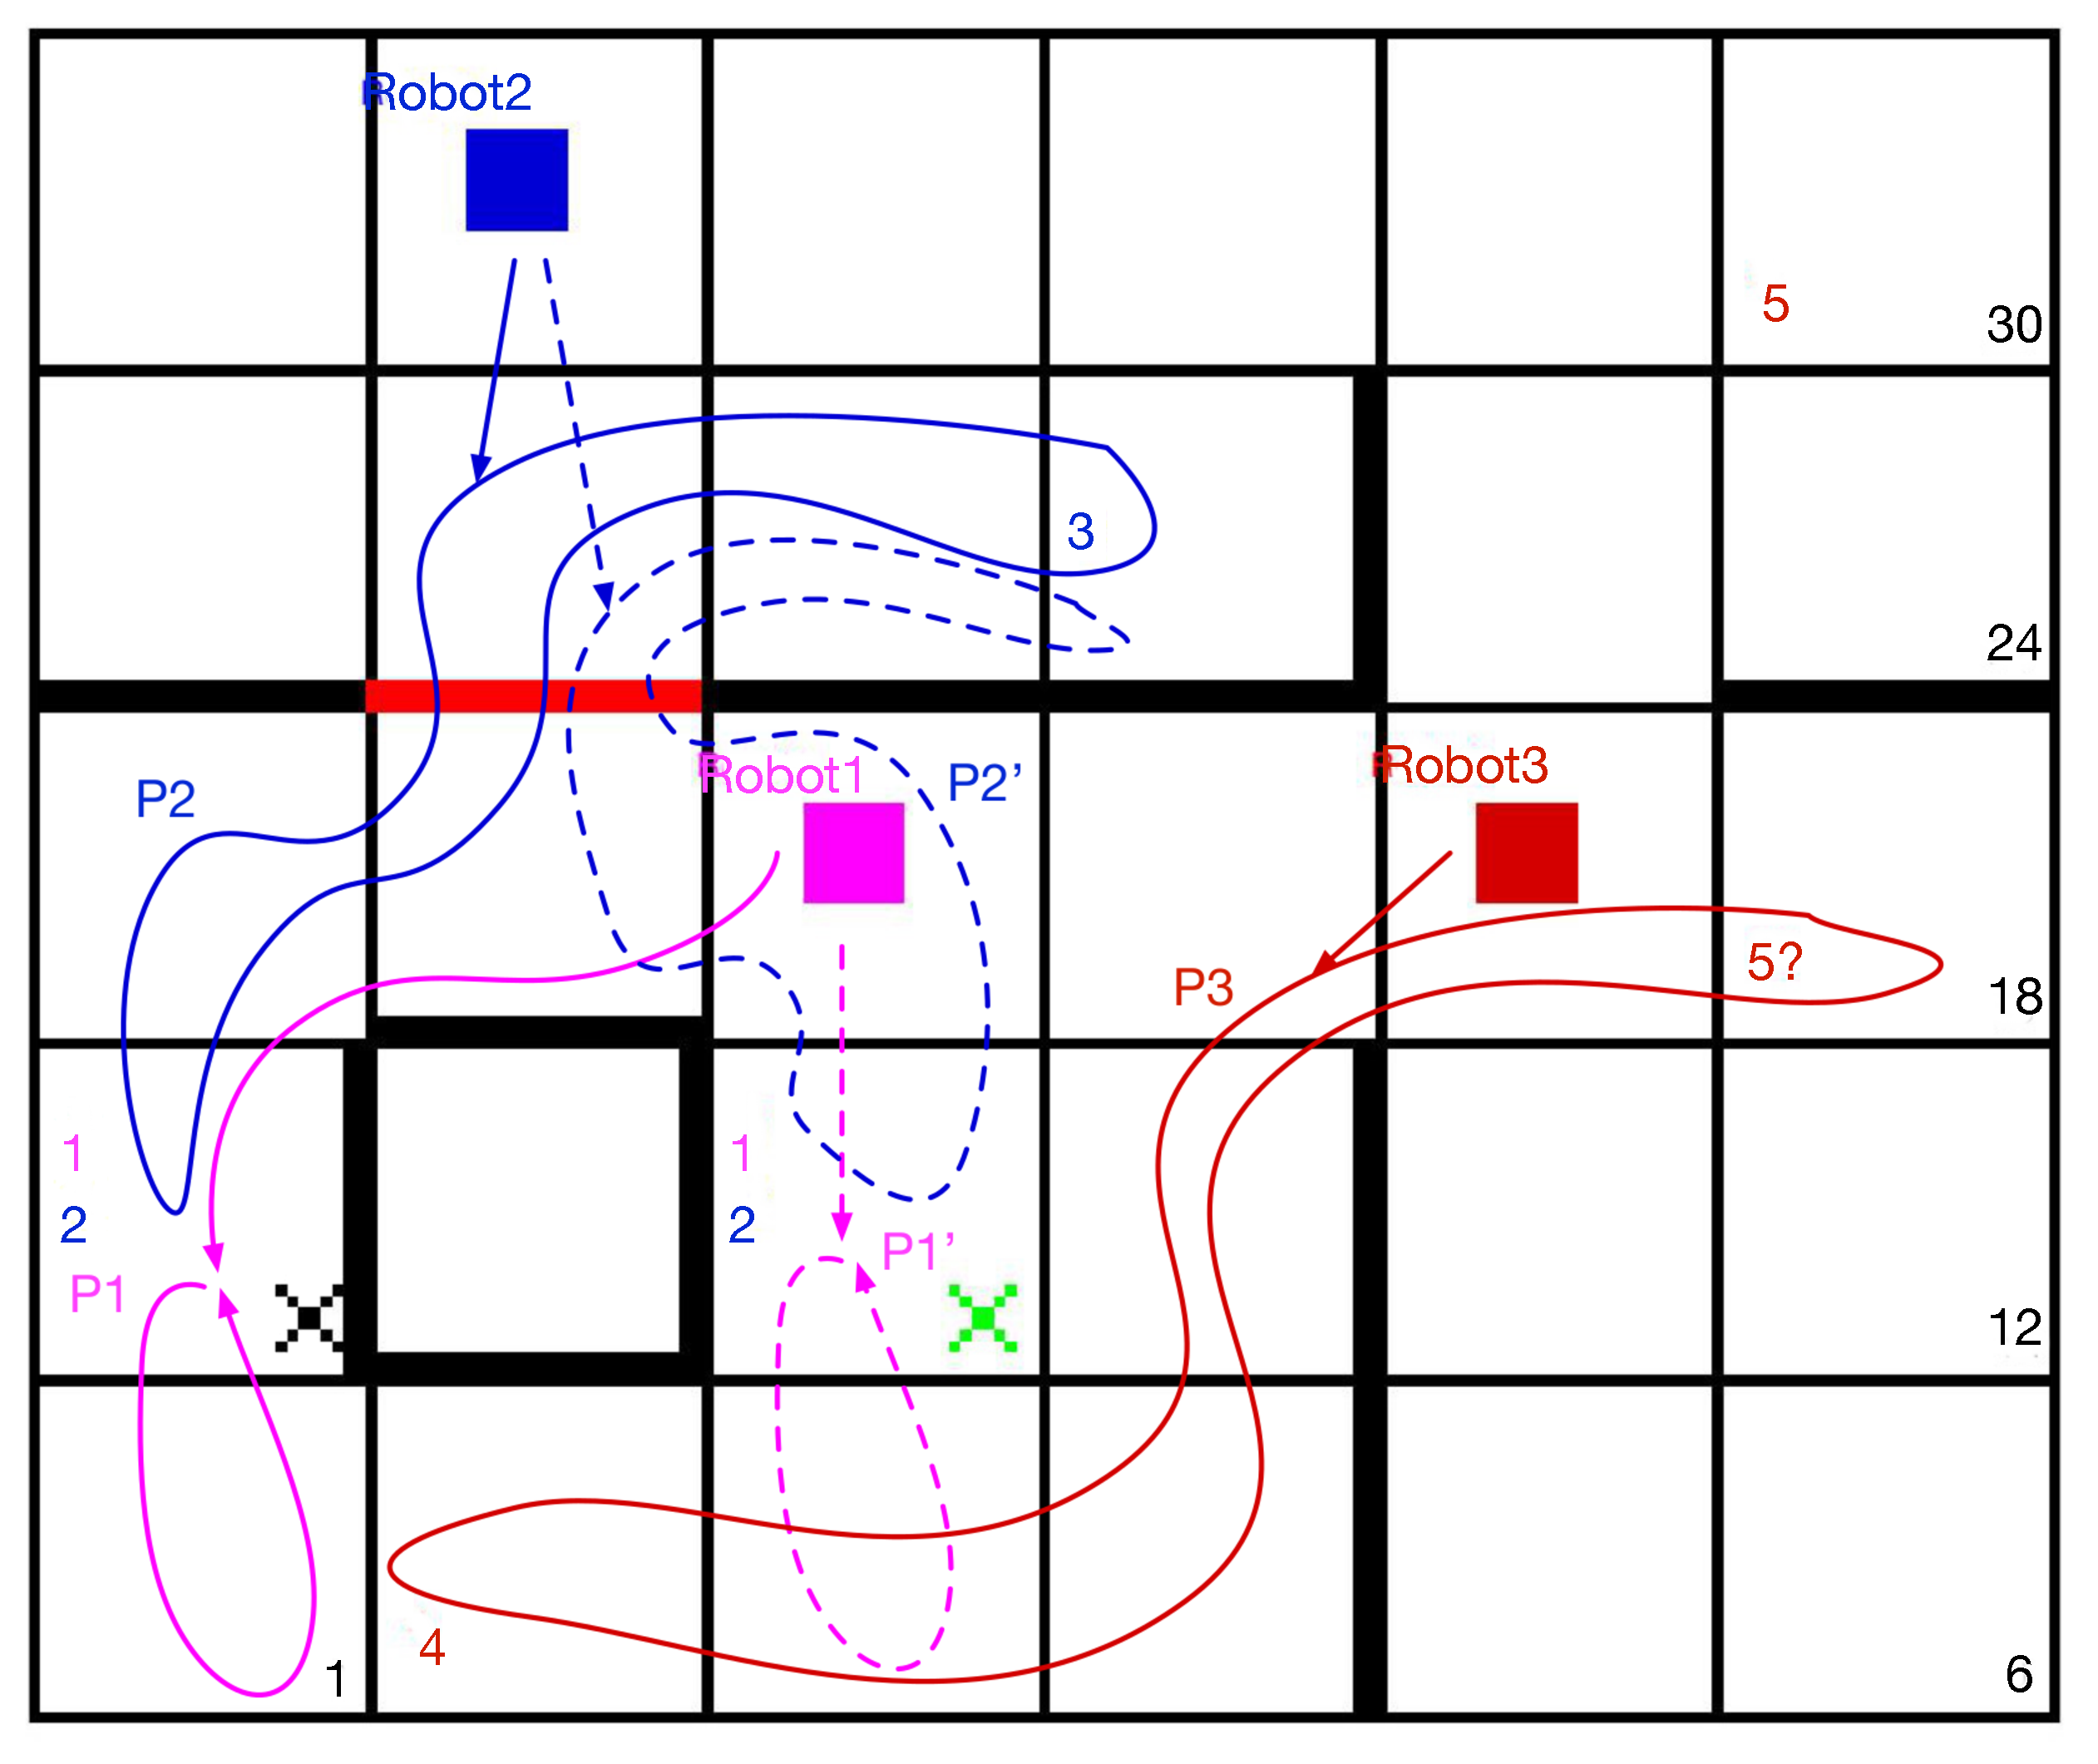
\includegraphics[width=1\linewidth]{Figures/arrows-v3.pdf}
\caption{\toolName\ usage scenario. \sergio{add another figure with a high-level explanation of this one}}
\label{fig:outputexample}
\vspace{-.5cm}
\end{center}
\end{figure}

%In~\cite{mapmaker17}  we have shown that our tool is able to perform a plan even in environments full of uncertainty.
%Thus, \toolName~ is able to compute a plan where other planners will not.
%However, the computation time and the number of actions to be performed by the robot that tries to follow a possible plan and detects a false evidence are normally greatly increased.
%This increasing is due to required re-computing that has to be performed when looking for a new possible plan.

%For checking its performance the tool was tested in different environments based on real-world scenarios.
%The model of the uncertainty of the environment was randomly created and matched with randomly models of the robots (service and synchronization locations and uncertainties).
%The performance of tool was evaluated in two Research Questions divided in three experiments (one for each kind of uncertainty defined for this project).
%The results are presented and discussed in~\cite{mapmaker17}.

%\textbf{Tool Validation}


